\chapter{Theoretische Grundlagen}

\section{Definition Schlüsselbegriffe}

\subsection{Künstliche Intelligenz}

KI - Künstliche Intelligenz – Definition wie solche, variieren mit der Zeit. Mitte 19. Jahrhundert verstand man unter der Begrifflichkeit „Digitalisierung“, 
eine Software, welcher Taschenrechner, Papier und Stift ersetzte. Inzwischen bedeutet Digitalisierung, die Entwicklung eines Systems, welches den Menschen ablöst 
und gleichzeitig sich selbst weiterentwickelt. Es lernt auf Basis bestehender Daten oder generiert selbständig neue Daten, um daraus zu lernen und seine 
eigenen Algorithmen zu verbessern. Bei vernetzter KI lernen die KI-Systeme voneinander2.
\newline

Der US-amerikanische Informatiker John McCarthy definierte das Wort Künstliche Intelligenz (1956) als die Wissenschaft und Technik der Herstellung der Maschinen. 
Die KI benutzt Computer, um menschliche Intelligenz um sich zu entwickeln. Sie muss sich nicht auf Methoden beschränken, die biologisch beobachtbar sind. 
Sie ist der rechnerische Teil der Fähigkeit, um Ziele in der Welt zu erreichen. Es treten bei Menschen, Tieren und einigen Maschinen unterschiedliche Arten der 
Intelligenz auf3
\newline

Intelligenz kommt aus dem lateinischen [intelligentia/intellegentia] und bedeutet so viel wie denken4. Deshalb ist die künstliche Intelligenz nicht exakt definiert, 
wird jedoch im Bereich Informatik verwendet und greift in der Regel auf intelligente Computerprogramme zurück. 
Bei der Definition des Begriffs wird auf die Abbildung des menschlichen Entscheidungsverhaltens verknüpft. 
In der Praxis sollen einfache Algorithmen dazu beitragen, ein intelligentes Verhalten zu plagiieren. Besonders wird in der KI das menschliche Verhalten geforscht, 
d.h. eine Maschine soll sich wie ein Mensch verhalten. Bislang war es eine Vision und konnte nicht umgesetzt werden. 
In der Theorie aber bedeutet die Künstliche Intelligenz, die Problemlösung des Computers, für deren Lösung eigentlich eine menschliche Intelligenz benötigt wird. 
\newline

Es wird zwischen einer starken und schwachen KI unterschieden. Die starke KI, auch genannt general AI, mechanisiert das komplette menschliche Denken. 
Diese Systeme sollen menschliche intellektuelle Fähigkeiten erreichen und diese sogar übertreffen. D.h. sie sollen nicht nur auf eine bestimmte Lösung eines 
Problems handeln, sondern sollen einen eigenen Antrieb, eine eigene Intelligenz sowie Flexibilität aufweisen. Bisher waren alle Forschungen für die schlaue KI 
erfolglos, jedoch hat sich die Welt seit 100 Jahren sehr weit entwickelt, wie z.B. das Internet oder elektrische Autos konstruiert. 
Falls es in der Zukunft dazu kommt, dann werden die KI-Fähigkeiten, logisches Denkvermögen, Entscheidungsvermögen, Planvermögen, Kommunikation in natürlicher Sprache 
aufweisen und diese kombinieren, um ein übergeordnetes Ziel zu erreichen5. Die schwache KI (weak KI) dagegen, wird für Lösungen konkreter Anwendungsprobleme und 
als Unterstützung des Denkprozesses benutzt. Diese ist mit mathematischen Methoden und Informatik ausgestattet, die für die jeweilige Anforderung entwickelt wurde.
Schwache KI verbirgt sich hinter Zeichen- oder Texterkennungsprogrammen, Navigationssystemen, Spracherkennungen oder hinter individuellen Anzeigen von Werbungen6.
Im menschlichen Körper verknüpfen sich circa 20 Milliarden Neuronen die Nervenzellen, die an einigen Stellen miteinander verbunden sind (Abbildung 2). 
Diese Verbindungen heißen Synapsen und sorgen für ein komplexes Netzwerk. Auf diese Art und Weise kann das Gehirn Informationen bearbeiten und ermöglicht dadurch
Fähigkeiten, wie das Gehen, Reden, Denken, Wahrnehmung. Die Funktionsweise der Künstlichen Intelligenz ähnelt dem menschlichen. Die Synapsen werden durch neuronale
Netzwerke ersetzt (Abbildung 1). Somit werden Informationen als Input eingegeben, im nächsten Schritt bearbeitet und das Ergebnis wird als Output
ausgespuckt. Dies nennt man das Algorithmussystem7.

\subsection{Machine learning}

Maschinelles Lernen ist ein Teilbereich der künstlichen Intelligenz und heißt zusammengefasst, dass die Roboter, Maschinen oder Computer, durch 
Daten und Informationen ernährt wird, die in Big-Data schweben. Sie werden nicht für bestimmte Aufgaben programmiert, sondern nutzen ausgefeilte Algorithmen, 
um aus enormen Big-Data-Mengen zu lernen. Der Einsatz von maschinellem Lernen begegnet uns bereits jeden Tag, wie z.B. personalisierte Werbungen auf den Handys,
Computer, Laptops, Produkte auf Amazon, Ebay oder Google. Sogar die Fotoalben auf den Handys können bereits Gesichter erkennen und Orte merken, 
wo die Bilder geschossen wurden. Je größer die Datenmenge ist, desto besser und leichter lernen sie12. Somit wird es dem System möglich automatisiert 
Zusammenhänge zu identifizieren, Wissen zu generieren, Algorithmen zu trainieren und unbekannte Muster zu erkennen (Abbildung 4).
\newline

Dadurch können neue und unbekannte Datensätze für Vorhersagen oder Prozessoptimierungen verwendet werden. Im Gegensatz zur manuellen Programmierung liegt 
bei Machine Learning der Schwerpunkt auf dem selbstständigen Lernen aus Daten und kann aus diesen Daten seinen Programmcode alleine erstellen. 
Das maschinelle Lernen kann Aufgaben wie, Werte auf Basis der analysierten Daten vorhersagen (bspw. Stromverbrauch oder Umsatzforecast), Wahrscheinlichkeiten 
für bestimmte Ereignisse (bspw. Kaufwahrscheinlichkeiten, Kündigungswahrscheinlichkeit) berechnen, Gruppen und Clustern in einem Datensatz erkennen, 
Zusammenhänge in Sequenzen erkennen, Dimensionen ohne große Informationen reduzieren und Geschäftsprozesse optimieren. Das Wort maschinelles Lernen wird oft mit 
den Begriffen Data Mining (ein analytischer Prozess, der eine autonome und effiziente Identifizierung und Beschreibung von interessanten Datenmustern aus großen 
Datenbeständen ermöglicht) und predictive Analytics (nutzt historische Datenquellen und erstellt aus diesen ein mathematisches Modell, mit dem sich zukünftige 
Ereignisse vorhersagen lassen) in Verbindung gebracht. Im Endeffekt nutzen diese die Verfahren des maschinellen Lernens. Machine Learning funktioniert nur,
wenn es durch einen Menschen mit vorbereiteten Trainingsdatensätzen trainiert wird, der von einem
\newline

Machine Learning Algorithmus nach Mustern und Zusammenhängen durchsucht wird. Das trainierte Modell wird für Bewertungen unbekannter Daten genutzt und können 
anhand Vorhersagen bessere Entscheidungen treffen. Das Ziel ist es, ohne menschliche Hilfen automatisch zu lernen. Bis eine bestimmte Qualität des Ergebnisses 
erreicht wird, werden mehrere Durchläufe des interaktiven Prozesses durchgeführt. Die Entwicklungsschleifen werden in der Praxis von einem Menschen bewertet.
Das maschinelle Lernen hat mehrere Arten, die folgendermaßen aufteilen: überwachtes Lernen (supervised Learning), unüberwachtes Lernen (unsupervised Learning), 
teilüberwachtes Lernen (semi-supervised Learning) und verstärkendes Lernen (reinforcement Learning). Das überwachte maschinelle Lernen trainiert anhand bekannter 
Daten, um Muster und Zusammenhänge zu lösen. Hierbei wird der Zusammenhang zu einer Zielvariable (eine Klasse oder ein nummerischer Wert) erlernt und versucht diese 
richtig vorherzusagen. Anhand dieses Lernprozesses werden für zukünftige oder unbekannte Daten Vorhersagen getroffen. Das unüberwachte Lernen dagegen hat keine 
bekannten Daten und muss durch Algorithmen eigenständig interessante sowie versteckte Gruppen und Muster erkennen. Der Unterschied zum überwachten Lernen ist, dass 
das unsupervised Learning keine Vorhersage für eine bestimmte Zielvariable berechnen kann. Beispiele für unüberwachtes maschinelles Lernen 
sind Clustering oder Association. In Teilüberwachtes Lernen dagegen geht es sowohl um Beispieldaten mit exakten Zielvariablen als auch um unbekannte Daten. 
Semi-supervised Machine Learning ist eine Mischung aus den oben genannten zwei Lernmethoden und beschäftigt sich ebenfalls mit bekannten Daten und Informationen, 
wie das überwachte Lernen. Der einzige Unterschied zwischen dem überwachten Lernen und teilüberwachten Lernen ist, dass das teilüberwachte Lernen mit weniger 
Daten an die Zielvariable kommt. Der Vorteil daran ist, dass mit einer geringeren Menge an bekannten Daten trainiert werden kann, da die Beschaffung 
der Beispieldaten sehr aufwendig und kostenintensiv werden kann. Hauptsächlich findet diese Lernmethode in der Bild- und Objekterkennung statt, wobei ein 
kleiner Datensatz von bekannten Bildern von Menschen erstellt wird. Das verstärkende Lernen, auch reinforcement Learning oder bestärkendes Lernen ist eine spezielle 
Form des maschinellen Lernens. Hier interagieren die Algorithmen mit der Umgebung und werden durch ein Belohnungssystem oder Kostensystem analysiert. 
So kann es selbstständig eine Strategie zur Lösung des Problems erlernen und die Belohnung maximieren. Die Belohnung ist in dem Fall keine Antwort zur Aktion, 
wie z.B. richtig oder falsch gehandelt, sondern eine positive oder negative Rückmeldung (Feedback). Das System lernt bestärkend durch die Kostenfunktion 
(welche Aktion ist zu welchem Zeitpunkt die richtige), die Belohnungsfunktion zu maximieren. Wichtiger Unterschied zwischen dem überwachten und 
unüberwachten Lernen und des vestärkenden Lernen ist, dass das verstärkende Lernen keine Beispieldaten benötigt, um zu lernen. Es ist eine große Hoffnung für KI-Forscher um Probleme, wie Fahren, Robotik Entwicklung einer generellen 
Künstlichen Intelligenz, zu lösen. Abbildung 5 zeigt auf, welche Einsatzgebiete es für Machine Learning gibt. Unüberwachtes Lernen ist mit den Bereichen 
Clusteranalyse und komplexe autonomes oder die generelle Künstliche Intelligenz zu lösen. Abbildung 5 zeigt auf, welche Einsatzgebiete es für Machine Learning gibt. 
Unüberwachtes Lernen ist mit den Bereichen Clusteranalyse und Dimensionsreduktion verbunden, d.h. z. B. Strukturen erkennen, Informationen 
komprimieren oder Segmentierung, während das überwachte Lernen mit den Gebieten Klassifikation (Objekt- /Texterkennung) und Prognose 
(Umsatzvorhersage, Wetter-/Nachfrageprognose) verbunden ist. Das verstärkende Lernen dagegen ist für Personalisierung und Werbung, Spiel KI, oder 
Verkehrssteuerung zuständig. Maschinelles Lernen hat in Customer-Relationship-Management ein breites Anwendungsgebiet, da der Wunsch aller 
Unternehmer die Kundenzufriedenheit zu steigern ist. CRM stellt dem Unternehmen die Funktion, Profitabilität Vorhersagen, Produktaffinitäten Berechnung, 
Kundensegmentierung für personalisierte Werbungen oder bevorstehende Abwanderungen, zur Verfügung13.

Abbildung 4: maschinelles Lernen
12 SAP (o. J.)

Abbildung 5: Anwendungsbereiche nach Arten


\subsection{Deep learning}

Deep Learning basiert als Teilbereich der Machine Learning auf künstliche neuronale Netze und Trainingsmethoden, bei denen die Maschinen große Datenmengen und 
Big Data analysieren und eine spezielle Methode der Informationsverarbeitung anwenden. Diese Methode ahnt der menschlichen Gehirnfunktion. 
Die Maschine generiert Wissen aus Erfahrung, sie enthält Informationen, analysiert sie und zieht ein Fazit daraus. Deep Learning stellt sicher, dass die 
Informationen für das Lernen bereitstehen, hat also keinen Einfluss auf das Ergebnis. Durch Deep Learning sind künstlich intelligente Maschinen in der Lage, 
zu prognostizieren und diese zu hinterfragen. In z. B. automatisiertes Fahren verwenden Entwickler Deep Learning für die automatische Erkennung von Objekten wie 
Stoppschilder, Ampeln, Brücken und Taxis, usw. Ebenfalls wird es für die Erkennung von Fußgängern verwendet, um Unfälle zu vermeiden. Deep Learning wird auch tiefe 
neuronale Netze genannt, da sie die Baustruktur der neuronalen Netze benutzt. Das Tiefe in dem Wort deep learning kommt von den mehreren Schichten in dem neuronalen 
Netzwerk. Künstliche neuronale Netze besitzen meistens nur zwei bis drei Schichten, tiefe Netze dagegen bis zu 150 Schichten. Neuronaler Faltungsnetzwerk ist eine Art
des Deep Learnings (Convolutional Neuroal Networks (CNN)) und faltet erlernte Merkmale mit Eingabedaten, wobei 2D-Faltungsebenen verwendet werden, 
die diese Baustruktur zur Verarbeitung von 2D-Daten geeignet macht. Das CNN arbeitet, indem es Merkmale aus Bildern extrahiert. Die Informationen werden nicht 
vorinstalliert, sondern sie werden darauf getrimmt, zu lernen. Durch diese automatisierte Funktion ist es dem Deep Learning möglich, für Aufgaben der Computer 
Vision, wie z. B. die Objektklassifikation, hervorragend zu erstellen. Mithilfe von verborgenen Ebenen, erlernt CNN unterschiedliche Merkmale eines Bildes 
zu erkennen. Durch jede weitere Ebene lernt das System Umrisse zu erkennen und die letzte Ebene erlernt komplexere Formen zu erkennen, die spezifisch zur Form 
des erkennenden Objekts passen. Jeder kennt es, bei Anmeldungen, Suchen o.ä. in Google den Captcha Test. Google will wissen, dass gerade durch eine Person gesucht 
wird und will daher einen Haken gesetzt haben. Dann kommt ein Pop-Up (Abbildung 9), dass alle Felder mit den oben genannten Gegenständen bzw. Personen ausgewählt 
werden müssen. Dabei wird dem Deep Learning geholfen, Gegenstände oder Personen zu erkennen. Google inc. will damit das autonome Fahren unterstützen, damit das 
Fahrzeug Personen, Brücken, Taxis, Ampeln, Fußgängerzonen, etc. erkennt16.

Häusser, P. (2018)
Abbildung 9: Google Captcha

\subsection{Neuronale Netze}

Künstliche neuronale Netze (KNN) sind Nachversuche des menschlichen Gehirns, also den biologischen Neuronalen Netzen. In beiden Fällen geht es hauptsächlich, 
um das Zusammenspiel aus den Nervenzellen, den Neuronen, und deren Verbindung zueinander (Synapsen). Das Ziel der künstlichen Neuronalen Netzen sind, Fortschritte 
im maschinellen Lernen anhand Big Data und Deep Learning zu erreichen. Ein Neuron besteht aus nur einem Informationsprozess und Informationsaspekt. Jedoch für 
eine gesamte oder komplexe Information müssen mehrere Neuronen verbunden werden, die als Synapsen benannt wurden. Ein neuronales Netz, künstlich oder biologisch, 
besteht also aus unendlichen Neuronen, die Signale empfangen und an andere Neuronen weiter übermitteln. Der Aufbau eines Neuronalen Netzes besteht grundsätzlich 
aus drei Ebenen, die im Folgenden kurz beschrieben werden14. Informationen fließen über Hidden Layer (Zwischenschicht) und/oder Output Layer (Ausgabeschicht). 
Der Output des einen Neurons ist der Input des nächsten. Die Neuronen erfolgen meistens schematisch horizontal, d.h. dass die Eingabeschicht auf der linken Seite, 
von den Zwischenschichten in der Mitte gefolgt und der Ausgabeschicht auf der rechten Seite angeordnet. Die Anzahl der Schichten ist eine wichtige Information. 
Wenn ein Netz 3 Schichten hat, so spricht man vom drei schichtigen Netz. Erstens: Input-Layer oder Eingabeschicht: In einem künstlichen neuronalen Netz ist der 
Input Layer der Startpunkt eines Informationsflusses. Die Informationen werden aufgenommen und am Ende der Schicht gewichtet und landet in der ersten Zwischenschicht. 
Während dessen gibt ein Neuron der Eingabeschicht die entsprechenden Daten an alle Neuronen der ersten Zwischenschicht weiter. Zweitens: Hidden Layer oder 
Zwischenschicht: Zwischen allen Input Layer und Output Layer befindet sich in jedem neuronalen Netz mindestens ein Hidden Layer. Wenn die neuronale Schicht groß ist,
hat es mehrere Zwischenschichten, auch genannt Aktivitätsschicht oder verborgene Schicht. Hierbei geht es um Deep Learning (Punkt 2.1.2.3). In der Regel ist die 
Anzahl der möglichen Schichten in einem neuronalen Netz unbegrenzt, jedoch bewirkt jede hinzugekommene Zwischenschicht einen Anstieg der Rechenleistung, die für 
den Betrieb notwendig ist. Drittens: Output Layer oder Ausgabeschicht: Die Ausgabeschicht dagegen liegt hinter den ersten zwei Schichten und bildet somit die letzte 
Schicht in einem Netzwerk. Hier sind die angeordneten Neuronen mit allen Neuronen der letzten Zwischenschicht verbunden. Das Output Layer stellt den Endpunkt des 
Informationsflusses dar und enthält das Ergebnis der Verarbeitung durch das neuronale Netzwerk. Wie funktioniert jedoch ein neuronales Netz? Neuronale Netze sind 
der Schlüssel für künstliche Intelligenz. Ein neuronales Netz kann ein Schachbrettmuster erkennen. Abbildung 6 zeigt uns ein Muster eines solchen Netzwerks. 
Oben hat es 4 Öffnungen, also die Eingabeschicht, hier fließen die Nervensignale durch bis sie an die Zwischenschicht, also weitere Neuronen, ankommt. Hier wird 
entschieden, ob ein Tennisball, also ein Nervensignal gefeuert wird, oder nicht. Um in der Zwischenschicht ein Tennisball auszulösen, bzw. ein Nervensignal
zu feuern, muss in der Eingabeschicht die Eingabe als „kein Schachbrettmuster“ (Abbildung 8) erfolgen. Wenn die Eingabe als Schachbrettmuster erkannt wird 
(Abbildung 6), dann ist das Ergebnis kein Tennisball, also die Neuronen feuern kein Nervensignal aus15.
 

13 Wuttke, L (o. J.)


Abbildung 7
Dusold, J. (2019)
Abbildung 6 Muster eines künstlichen neuronalen Netzes


\section{Aktueller Stand der KI in der Arbeitswelt}

Deutsche Unternehmen investieren vermehrt in intelligente Systeme, sei es Computerprogramme oder Logistiksysteme, das Ziel dabei ist die Modernisierung und 
Optimierung. Jedoch tun sich Unternehmen bei der Implementierung solcher Systeme schwer. Meistens fehlt es an personellen Ressourcen, finanziellen Ressourcen 
oder Zeit. Die Erkenntnis ist aber, dass nach der Einsetzung viele Unternehmen produktiver gestaltet sind. So werden tägliche menschliche Fehler vermieden und 
individuelle Prozessanalysen entworfen. Künstliche Intelligenz wird als Marketingtool, Produktion und Instandhaltung, zur Optimierung interner Prozesse oder
im Kundendienst verwendet. In der Entwicklung der Künstlichen Intelligenz ist Deutschland weit fortgeschritten, viele Unternehmen, die solche Systeme anbieten 
haben ihren Sitz in Deutschland. Bei Unternehmen mit einer Größe von 20 bis 99 Mann sehen 60 \% die Künstliche Intelligenz als wichtige Zukunftstechnologie. 
Bei Großunternehmen liegt diese Quote bei 90 \%. Nichtsdestotrotz benutzen lediglich 8 \% KI-Anwendungen. Im Gegensatz hierzu planen viele Unternehmen KI-Anwendungen
aktiv einzusetzen\footnote{https://www.lsa-partnernetzwerk.de/studie-aktueller-stand-von-kuenstliche-intelligenz-in-der-deutschen-wirtschaft/}.\cite{wagener2019künstliche}
\newline

\subsection{Künstliche Intelligenz als Marketingtool}



\subsection{Künstliche Intelligenz in der Produktion und Instandhaltung}



\subsection{Künstliche Intelligenz als Dienstleister}


\section{Chancen und Risiken}


\section{Ethische Problemsituationen}


\section{Auswirkungen der KI auf den Arbeitsmarkt}

\subsection{Auswirkungen der Künstlichen Intelligenz im Marketing}

\subsection{Auswirkungen der Künstlichen Intelligenz in der Produktion und Instandhaltung}

\subsection{Auswirkungen der Künstlichen Intelligenz in der Dienstleistung}


\begin{figure}
	\caption[Architektur]{Architektur}
	\centering
	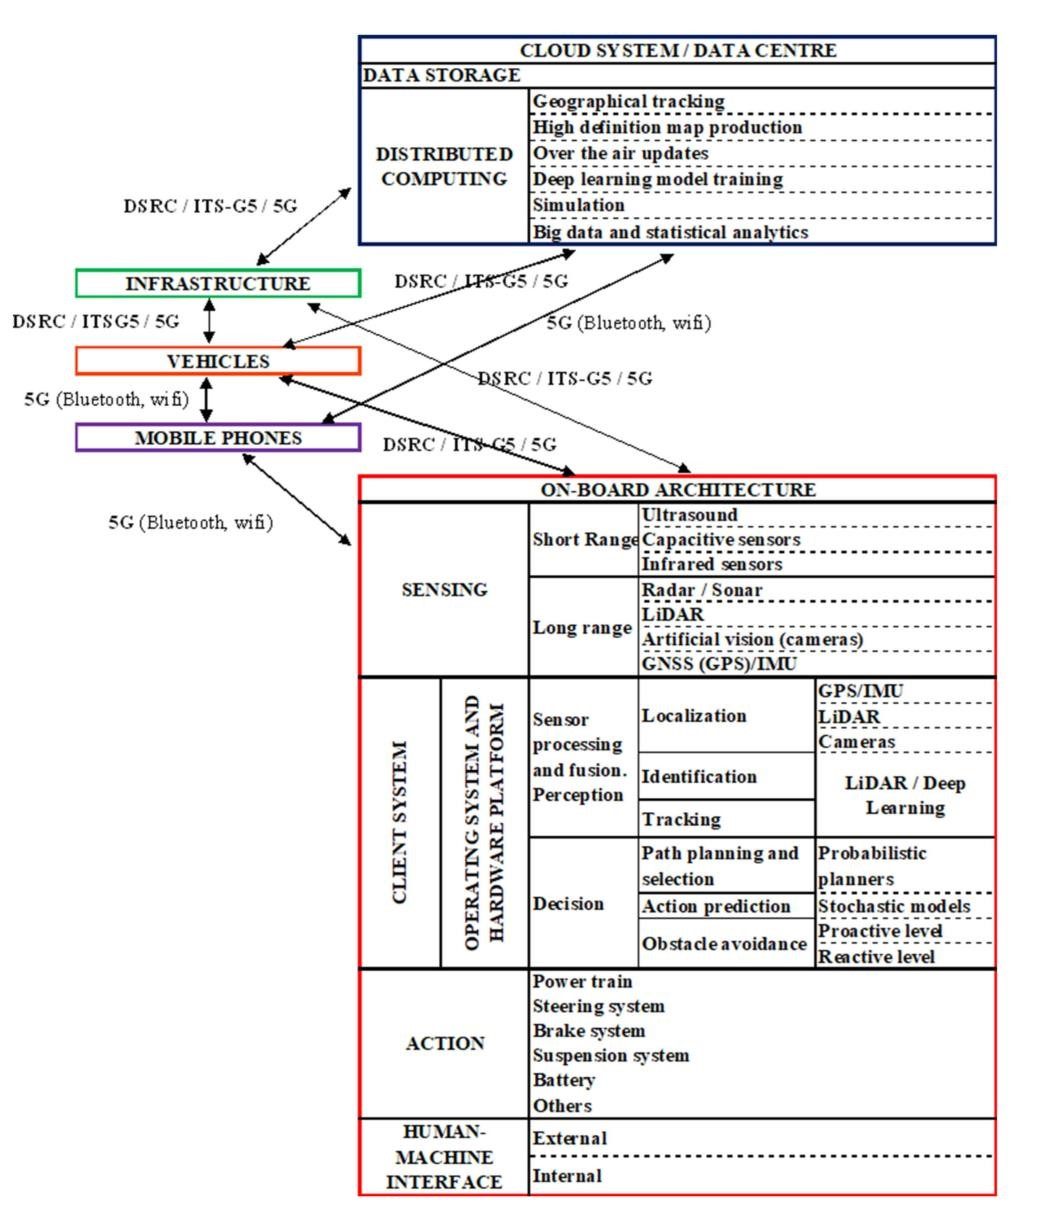
\includegraphics[]{assets/figures/Architektur.jpg}
	\begin{flushleft}
		Quelle: Martínez-Díaz, M./Soriguera, F./Pérez, I., Autonomous driving: a bird's eye view, 2019, S. 564.	
	\end{flushleft}														
\end{figure}

Stet clita kasd gubergren, no sea takimata sanctus est Lorem ipsum dolor sit amet Acceptance of autonomous driving will depend on how far a consensus on these norms can be found, first among experts, then in society at large. 
One ethical condition, however, should be crucial: in no case should the ethical algorithms be put in practice as nontransparent black boxes. 
The built-in norms should, as far as possible, be understood and commonly shared.

\chapter{Methode und Analyse}

\section{Untersuchungsmethode}

Lorem ipsum dolor sit amet, consetetur sadipscing elitr, sed diam nonumy eirmod tempor invidunt ut labore et dolore magna aliquyam erat, sed diam voluptua. 
At vero eos et accusam et justo duo dolores et ea rebum. 
Stet clita kasd gubergren, no sea takimata sanctus est Lorem ipsum dolor sit amet. 
Automation in cars has a long history.  Lorem ipsum dolor sit amet, consetetur sadipscing elitr, sed diam nonumy eirmod tempor invidunt ut labore et dolore magna aliquyam erat, sed diam voluptua. 
At vero eos et accusam et justo duo dolores et ea rebum.\footnote{Vgl. Baumann, M. F. u. a., Taking responsibility: A responsible research and innovation (RRI) perspective on insurance issues of semi-autonomous driving, 2019, S. 558.} 
Stet clita kasd gubergren, no sea takimata sanctus est Lorem ipsum dolor sit amet Acceptance of autonomous driving will depend on how far a consensus on these norms can be found, first among experts, then in society at large. 
One ethical condition, however, should be crucial: in no case should the ethical algorithms be put in practice as nontransparent black boxes. 
The built-in norms should, as far as possible, be understood and commonly shared.


\section{Literaturanalyse}

\begin{table}[h]
	\caption{Tolle Tabelle}
	\centering
	\begin{tabular}{ | c | c | c | } 
		\hline
		cell1 & cell2 & cell3 \\ 
		cell4 & cell5 & cell6 \\ 
		cell7 & cell8 & cell9 \\ 
		\hline
	\end{tabular}
	\begin{flushleft}
		Quelle: Martínez-Díaz, M./Soriguera, F./Pérez, I., Autonomous driving: a bird's eye view, 2019, S. 564.	
	\end{flushleft}	
\end{table}

Lorem ipsum dolor sit amet, consetetur sadipscing elitr, sed diam nonumy eirmod tempor invidunt ut labore et dolore magna aliquyam erat, sed diam voluptua. 
At vero eos et accusam et justo duo dolores et ea rebum. 
Stet clita kasd gubergren, no sea takimata sanctus est Lorem ipsum dolor sit amet. 
Automation in cars has a long history.  Lorem ipsum dolor sit amet, consetetur sadipscing elitr, sed diam nonumy eirmod tempor invidunt ut labore et dolore magna aliquyam erat, sed diam voluptua. 
At vero eos et accusam et justo duo dolores et ea rebum.\footnote{Vgl. Baumann, M. F. u. a., Taking responsibility: A responsible research and innovation (RRI) perspective on insurance issues of semi-autonomous driving, 2019, S. 558.} 
Stet clita kasd gubergren, no sea takimata sanctus est Lorem ipsum dolor sit amet Acceptance of autonomous driving will depend on how far a consensus on these norms can be found, first among experts, then in society at large. 
One ethical condition, however, should be crucial: in no case should the ethical algorithms be put in practice as nontransparent black boxes. 
The built-in norms should, as far as possible, be understood and commonly shared.

\section{Diskussion der These an Hand der Literatur}

Lorem ipsum dolor sit amet, consetetur sadipscing elitr, sed diam nonumy eirmod tempor invidunt ut labore et dolore magna aliquyam erat, sed diam voluptua. 
At vero eos et accusam et justo duo dolores et ea rebum.\footnote{Vgl. Baumann, M. F. u. a., Taking responsibility: A responsible research and innovation (RRI) perspective on insurance issues of semi-autonomous driving, 2019, S. 558.} 
Stet clita kasd gubergren, no sea takimata sanctus est Lorem ipsum dolor sit amet. 
Automation in cars has a long history.  Lorem ipsum dolor sit amet, consetetur sadipscing elitr, sed diam nonumy eirmod tempor invidunt ut labore et dolore magna aliquyam erat, sed diam voluptua. 
At vero eos et accusam et justo duo dolores et ea rebum. 
Stet clita kasd gubergren, no sea takimata sanctus est Lorem ipsum dolor sit amet Acceptance of autonomous driving will depend on how far a consensus on these norms can be found, first among experts, then in society at large. 
One ethical condition, however, should be crucial: in no case should the ethical algorithms be put in practice as nontransparent black boxes. 
The built-in norms should, as far as possible, be understood and commonly shared.


Lorem ipsum dolor sit amet, consetetur sadipscing elitr, sed diam nonumy eirmod tempor invidunt ut labore et dolore magna aliquyam erat, sed diam voluptua. 
At vero eos et accusam et justo duo dolores et ea rebum. 
Stet clita kasd gubergren, no sea takimata sanctus est Lorem ipsum dolor sit amet. 
Automation in cars has a long history.  Lorem ipsum dolor sit amet, consetetur sadipscing elitr, sed diam nonumy eirmod tempor invidunt ut labore et dolore magna aliquyam erat, sed diam voluptua. 
At vero eos et accusam et justo duo dolores et ea rebum.\footnote{Vgl. Baumann, M. F. u. a., Taking responsibility: A responsible research and innovation (RRI) perspective on insurance issues of semi-autonomous driving, 2019, S. 558.}
Stet clita kasd gubergren, no sea takimata sanctus est Lorem ipsum dolor sit amet Acceptance of autonomous driving will depend on how far a consensus on these norms can be found, first among experts, then in society at large. 
One ethical condition, however, should be crucial: in no case should the ethical algorithms be put in practice as nontransparent black boxes. 
The built-in norms should, as far as possible, be understood and commonly shared.

\section{Konsequenzen}

Lorem ipsum dolor sit amet, consetetur sadipscing elitr\footnote{Vgl. Baumann, M. F. u. a., Taking responsibility: A responsible research and innovation (RRI) perspective on insurance issues of semi-autonomous driving, 2019, S. 558.}, sed diam nonumy eirmod tempor invidunt ut labore et dolore magna aliquyam erat, sed diam voluptua. 
At vero eos et accusam et justo duo dolores et ea rebum. 
Stet clita kasd gubergren, no sea takimata sanctus est Lorem ipsum dolor sit amet. 
Automation in cars has a long history.  Lorem ipsum dolor sit amet, consetetur sadipscing elitr, sed diam nonumy eirmod tempor invidunt ut labore et dolore magna aliquyam erat, sed diam voluptua. 
At vero eos et accusam et justo duo dolores et ea rebum. 
Stet clita kasd gubergren, no sea takimata sanctus est Lorem ipsum dolor sit amet Acceptance of autonomous driving will depend on how far a consensus on these norms can be found, first among experts, then in society at large. 
One ethical condition, however, should be crucial: in no case should the ethical algorithms be put in practice as nontransparent black boxes. 
The built-in norms should, as far as possible, be understood and commonly shared.